% flashcards-title: Liquid level against a milliliter scale
% flashcards-desc: An upright rounded vessel holds shaded liquid. Along its right side runs a vertical scale labeled from zero to eighty milliliters at every ten, with five equal small steps between neighboring labels. The flat top surface of the liquid lines up with the second small mark above the sixty label, and a dashed guide joins the liquid surface to that point on the scale.
\documentclass[dvisvgm,tikz,border=8pt]{standalone}
\usepackage{tikz}
\usetikzlibrary{arrows.meta,calc,positioning}
\definecolor{DeckInk}{HTML}{172A3A}
\definecolor{DeckAccent}{HTML}{176B87}
\definecolor{DeckWarm}{HTML}{D97706}
\definecolor{DeckMuted}{HTML}{667784}
\definecolor{DeckPaper}{HTML}{F7FAFC}
\tikzset{
  every node/.style={font=\sffamily, text=DeckInk},
  object/.style={draw=DeckInk, line width=1.1pt, fill=DeckPaper},
  primary/.style={draw=DeckAccent, line width=1.5pt},
  boundary/.style={draw=DeckAccent, line width=1.5pt, dashed, rounded corners=6pt},
  guide/.style={draw=DeckMuted, line width=0.9pt, dashed},
  dimension/.style={{Stealth[length=3.2mm,width=2.2mm]}-{Stealth[length=3.2mm,width=2.2mm]}, draw=DeckWarm, line width=1.2pt},
  motion/.style={-{Stealth[length=3.5mm,width=2.5mm]}, draw=DeckAccent, line width=1.5pt, dashed},
}

\begin{document}
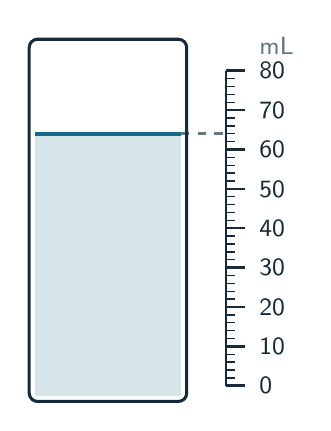
\begin{tikzpicture}[x=1cm,y=1cm]
  % Liquid
  \fill[DeckAccent!18] (0.07,0.07) rectangle (1.93,3.4);
  % Guide from surface to scale, painted before the level line
  \draw[guide] (1.93,3.4) -- (2.5,3.4);
  % Liquid surface
  \draw[primary] (0.07,3.4) -- (1.93,3.4);
  % Vessel
  \draw[object, fill=none, rounded corners=3pt] (0,0) rectangle (2,4.6);
  % Scale
  \draw[DeckInk, line width=1.0pt] (2.5,0.2) -- (2.5,4.2);
  \foreach \y in {0.3,0.4,...,4.15}
    \draw[DeckInk, line width=0.5pt] (2.5,\y) -- (2.62,\y);
  \foreach \k in {0,...,8}{
    \draw[DeckInk, line width=0.9pt] (2.5,0.2+0.5*\k) -- (2.74,0.2+0.5*\k);
    \node[font=\sffamily\small, anchor=west] at (2.8,0.2+0.5*\k) {\pgfmathparse{int(10*\k)}\pgfmathresult};
  }
  \node[text=DeckMuted, font=\sffamily\small, anchor=west] at (2.8,4.52) {mL};
\end{tikzpicture}
\end{document}
